% This is samplepaper.tex, a sample chapter demonstrating the
% LLNCS macro package for Springer Computer Science proceedings;
% Version 2.21 of 2022/01/12
%
\documentclass[runningheads]{llncs}
%
\usepackage[T1]{fontenc}
% T1 fonts will be used to generate the final print and online PDFs,
% so please use T1 fonts in your manuscript whenever possible.
% Other font encondings may result in incorrect characters.
%
\usepackage{graphicx}
% Used for displaying a sample figure. If possible, figure files should
% be included in EPS format.
%
% If you use the hyperref package, please uncomment the following two lines
% to display URLs in blue roman font according to Springer's eBook style:
%\usepackage{color}
%\renewcommand\UrlFont{\color{blue}\rmfamily}
%
\usepackage{amsmath}
\newtheorem{axiom}{Axiom}
\newtheorem{invariant}{Invariant}
\usepackage{chgtrk}
\newCTcontributor{Son}
\newCTcontributor{Colin}
\usepackage[colour]{lstEventB}
\usepackage{colourSoton}
\usepackage{hyperref}
\hypersetup{
  colorlinks=true,
  linkcolor = sotonMarine3,
  urlcolor=sotonMarine1,
  citecolor=sotonHorizon3
}
\begin{document}
%
% \title{SCXML Run-To-Completion Semantics\thanks{}}
\title{Formal Language Semantics for Triggered Enable Statecharts with a Run-to-Completion Scheduling}
\titlerunning{Formal Semantics for Triggered Statecharts}
%
%\titlerunning{Abbreviated paper title}
% If the paper title is too long for the running head, you can set
% an abbreviated paper title here
%
\author{
Karla Vanessa Morris Wright\inst{1}\orcidID{0000-0002-0146-3176} \and
Thai Son Hoang \inst{2}\orcidID{0000-0003-4095-0732} \and
Colin Snook\inst{2}\orcidID{0000-0002-0210-0983} \and
Michael Butler\inst{2}\orcidID{0000-0003-4642-5373}
}
%
\authorrunning{K. Morris et al.}
% First names are abbreviated in the running head.
% If there are more than two authors, 'et al.' is used.
%
%
% the affiliations are given next; don't give your e-mail address
% unless you accept that it will be published
\institute{
	Sandia National Laboratories, 
	7011 East Avenue Livermore, California 94550, USA\\
	\email{knmorri@sandia.gov\footnote{Corresponding author, telephone: +1(925) 294-3287}}
	\and
	ECS, University of Southampton,
	Southampton SO17 1BJ, United Kingdom\\
	\email{\{cfs,t.s.hoang,m.j.butler\}@soton.ac.uk}
}
%
\maketitle              % typeset the header of the contribution
%
\begin{abstract}
The increased complexity of high-consequence digital system designs with intricate interactions between numerous components has placed a greater need on ensuring that the design satisfies its intended requirements. This digital assurance can only come about through rigorous mathematical analysis of the design. This manuscript provides a detailed description of a formal language semantics that can be used for modeling and verification of systems. We use Event-B to build a formalised semantics that supports the construction of triggered enable statecharts with a run-to-completion scheduling. Rodin has previously been used to develop and analyse models using this semantics. 

\keywords{Run-To-Completion  \and statecharts \and Formal Semantics \and SCXML \and Event-B}
\end{abstract}
%
%
%
%\section{Plan}

% \begin{itemize}
%     \item Semantics for run to completion (SCXML is an example)
% \begin{itemize}
%     \item Extenal/Internal Trigger
%     \item Raising a sequence of internal triggers
%     \item Run-to-completion steps (completed flag)
% \end{itemize}
% \item Semantics for Statemachine
% \item Event-Triggered Statemachine = Statemachine + Triggers
% \end{itemize}


\section{Introduction}
We formalise the semantics of refinement in SCXML by modelling, in Event-B,
\begin{itemize}
	\item the structure and behaviour of abstract SCXML models,
	\item the structure, behaviour of refined SCXML models and their relationship to abstract models.
	\item We then refine the latter to remove verification artifacts and show that it is no different to the abstract model and hence SCXML refinement can be applied iteratively.
\end{itemize}

Since SCXML consists of a state-chart behaviour superimposed with a 'run to completion' execution semantics, we formalise the refinement of these two parts separately and then compose the two definitions to obtain the complete SCXMl refinement semantics.
% !TEX root = ../main.tex

\section{Background}
\label{sec:background}
 
% !TEX root = ../main.tex

\subsection{Event-B}
\label{sec:eventb}

\EventB~\cite{abrial10:_model_event_b,hoang13:_introd_event_b_model_method} is a formal method for system
design.  It uses \emph{refinement} to introduce system details gradually into the
formal model.  An \EventB model contains two parts: \emph{contexts} and \emph{machines}. 
Contexts contain \emph{carrier sets}, \emph{constants}, and \emph{axioms} constraining 
the carrier sets and constants.  Machines contain \emph{variables} |v|, \emph{invariants} |I(v)| 
constraining the variables, and \emph{events}. An event consists of a guard 
denoting its enabled-condition and an action defining the value of variables after the event is executed.  
In general, an event |e| has the form: |any t where G(t, v) then S(t, v) end| where |t| 
are the event parameters, |G(t, v)| is the guard of the event, and |S(t, v)| is the action of the event.
% \begin{center}
  % |any t where G(t, v) then S(t, v) end|
%& \inlineevent{\Be}{}{\Bt}{G(\Bt,\Bv)}{}{S(\Bt,\Bv)}
% \end{center}
%In the case where the event has no parameters, we use the following form
%\begin{center}
%  |when G(v) then S(v) end|
%%& \inlineevent{\Be}{}{}{G(\Bv)}{}{S(\Bv)}~,
%\end{center}
% and when the event has no parameters and no guard, we use
% \begin{center}
%   |begin S(v) end|
% %& \inlineevent{\Be}{}{}{}{}{S(\Bv)}~.
% \end{center}
%The action of an event comprises of one or more assignments, each of them has one of the following forms: (1) |v := E(t, v)|, (2) |v :: E(t, v)|, and (3) |v :∣ P(t, v)|.  Assignments of form (1) are deterministic, assign the value of expression |E(t, v)| to |v|.  Assignments of forms (2) and (3) are non-deterministic. (2) assigns any value from the set |E(t,v)| to |v|, while (3) assigns any value satisfied predicate |P(t,v)| to |v|.
%A machine in \EventB corresponds to a transition system
%where \emph{variables} represent the states and \emph{events} specify
%the transitions.  Note that invariants |I(v)| are inductive, i.e., they must be \emph{maintained} by all events. This is more strict than general safety properties which hold for all reachable states of the \EventB machine.  
% This is also the difference between verifying the consistency of \EventB machines using theorem proving and model checking (e.g., \PROB) techniques: model checkers explore all reachable states of the system while interpreting the invariants as safety properties.  

Machines can be refined by adding more details.  Refinement can be done by extending the machine 
to include additional variables (\emph{superposition refinement}) representing new features of 
the system, or by replacing some (abstract) variables by new (concrete) variables (\emph{data refinement}).  
% More information about \EventB can be found
% in~\cite{hoang13:_introd_event_b_model_method}.
Refinement in \EventB is reasoned on an event basis.  
A (concrete) event |f| refines an (abstract) event |e| if whenever |f| is enabled then |e| is also enabled (guard strengthening), and the action of |f| is the same or equivalent to |e| (where equivalence is given by some relationship defined in the invariants). 
New events are said to refine `skip' (an implicit abstract event that did nothing), and therefore do not alter abstract variables.
 More information about \EventB refinement can be
found in~\cite{abrial10:_model_event_b}.
\EventB is supported by the Rodin Platform (Rodin\footnote{An extensible toolkit which includes 
facilities for modelling, verifying the consistency of models using theorem proving and model 
checking techniques, and validating models with simulation-based approaches.})~\cite{abrial10:_rodin}.

\hl{Proof obligations are generated to ensure the consistency of
  \mbox{\EventB} models.  An important proof obligation in
  \mbox{\EventB} is invariant preservation to prove that safety
  properties (encoded as invariants of the models) will not be
  violated for any reachable states.  In this paper, we also make use
  of other proof obligations in \mbox{\EventB} such as (relative)
  deadlock-freeness and (conditional) event convergence to construct
  our proof of liveness properties under some fairness
  assumptions.%
}

\hl{%
  For the trace semantics corresponding to \mbox{\EventB} machines and
  the interpretation of LTL properties over traces, we refer the readers
  to \mbox{\cite{hoang2016ltl}}.  Here, we recall the notation for
  fairness assumptions underlying event-based formalisms such as
  \mbox{\EventB~\cite{lamport1977proving,hudon16:_unit_b_method}}. Given
  an event \mbox{\EventBInline{e}}, a weak-fairness assumption
  \mbox{\EventBInline{WF(e)}} states that if \mbox{\EventBInline{e}}
  is enabled continually, then it must occur infinitely often.
  Similarly, a strong-fairness assumption \mbox{\EventBInline{SF(e)}}
  states that if \mbox{\EventBInline{e}} is enabled infinitely often,
  then it must occur infinitely often. Formally,
}
\begin{center}
  \EventBInline{WF(a)  <=> (FG enabled(e) => GF [e])}, and

  \EventBInline{SF(a)  <=> (GF enabled(e) => GF [e])},
\end{center}
\hl{%
  where \mbox{\EventBInline{G}} and \mbox{\EventBInline{F}} are the
  temporal operators denoting \emph{globally}, and \emph{finally},
  respectively; and \mbox{\EventBInline{enabled(e)}} denotes that
  event \mbox{\EventBInline{e}} is enabled and
  \mbox{\EventBInline{[e]}} denotes an occurrence of event
  \mbox{\EventBInline{e}}.
}
% In \EventB the run to completion pseudocode of Listing~\ref{lst:scxml-r2c} could be represented (somewhat abstractly) as shown in Listing~\ref{lst:eventb-r2c}.
% \begin{lstlisting}[caption={Run to completion pseudocode in \EventB},label={lst:eventb-r2c}, language=Event-B, escapechar=|, frame=single, float=t]
%  FireUntriggered // Fire  enabled un-triggered transitions
% when
%     UC = FALSE // Has not yet completed firing un-triggered transitions
%     untriggered() /= {}
% then
%     execute(untriggered()) // Execute enabled un-triggered transitions
% end
% UntriggeredCompleted // Un-triggered transitions are completed
% when
%     UC = FALSE // Has not yet completed firing un-triggered transitions
%     untriggered() = {} // No more enabled un-triggered transitions
% then
%     UC = TRUE // Complete firing un-triggered transitions
% end
% FireInternallyTriggered // Fire an internal trigger
% when
%     UC = TRUE // Complete firing un-triggered transitions
%     IQ /= {} // The internal triggers queue is non-empty
% then
%     execute(IQ.dequeue) // Execute and dequeue from the internal triggers queue
%     UC := FALSE // Re-enable firing of un-triggered transitions
% end
% FireExternallyTriggered // Fire an external trigger
% when
%     UC = TRUE // Complete firing un-triggered transitions
%     IQ = {} // The internal trigger queue is empty
%     EQ /= {} // The external trigger queue is non-empty
% then
%     execute(EQ.dequeue)  // Execute and dequeue from the external triggers queue
%     UC := FALSE // Re-enable firing of un-triggered transitions
% end
% \end{lstlisting}	
% Here, |IQ| and |EQ| are queues of internally and externally, raised triggers, |untriggered| selects a set of currently enabled un-triggered transitions, |dequeue| retrieves the next trigger from the given queue and selects the set of transitions that become enabled by it and |execute| fires the given set of transitions. 
% Note that this is an abstract representation where each event (|FireUntriggered|, |FireInternallyTriggered|, and |FireExternallyTriggered|) would be specialised to select a particular set of transitions that can be fired in parallel and |execute()| would be replaced by actions that encode the state changes made by those transitions.
% Representing the condition \textbf{untriggered\_enabled} (Line 3 in Listing~\ref{lst:scxml-r2c}) is cumbersome since we would need to write a conjunction of all the possible un-triggered guards. Instead we introduce a dummy un-triggered event that is only fired when no other selection of un-triggered transitions are available and sets a boolean flag, |UC|, to indicate that none of the real un-triggered events was fired and a trigger needs to be consumed.
 
% Note that causing all of the
% transitions to simultaneously and atomically fire for each event is a
% further semantic choice.  Transitions associated with |FireUntriggered|,
% |FireInternallyTriggered|, and |FireExternallyTriggered| might
% just as well fire separately in a non-deterministic order, or by use
% of a per-transition priority, fire in a predetermined order.  Each
% choice has realistic exemplars in the physical world, and to some
% degree, the choice is arbitrary.  The argument in favour of the
% parallel atomic transitions chosen here is pragmatic: the resulting
% representation in \EventB is more terse.

%%% Local Variables:
%%% mode: latex
%%% TeX-master: "../main"
%%% End:

% !TEX root = ../main.tex

\subsection{UML-B State-machines}
\label{sec:iumlb}

\UMLB~\cite{said15:umlbSosym,snook14:iumlbStatem,snook06umlbTosem} provides a diagrammatic modelling notation for \EventB in the form of state-machines and class diagrams. 
The diagrammatic models relate to an \EventB machine and generate or contribute to parts of it. 
For example a state-machine will automatically generate the \EventB data elements (sets, constants, axioms, variables, and invariants) to implement the states. 
Transitions contribute further guards and actions representing their state change, to the events that they elaborate.  
State-machines are typically refined by adding nested state-machines to states.
% Figure~\ref{fig:iumlb-sm} shows an example of a simple state-machine with two states.
% \begin{figure}[!h]
% 	\vspace{-.5cm}
% 	\centering
% 	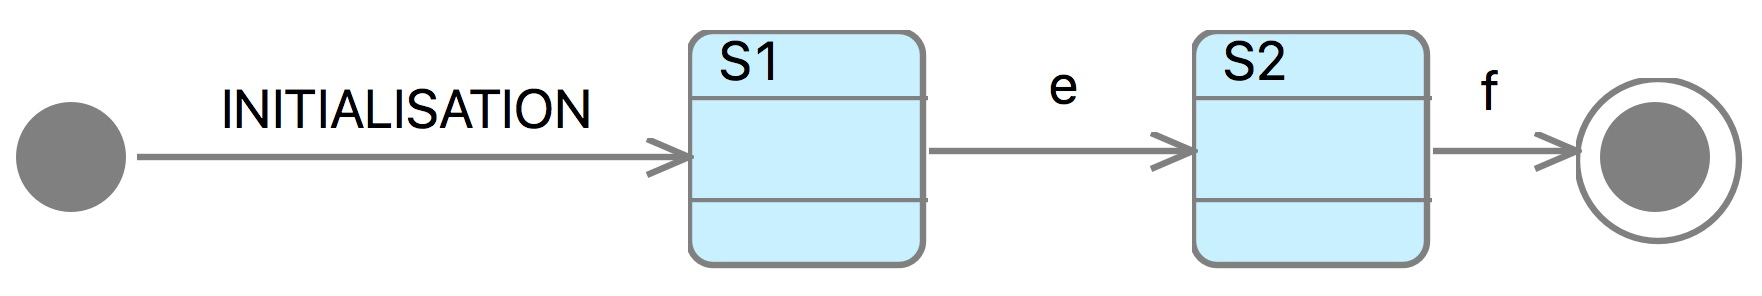
\includegraphics[width=0.6\textwidth]{figures/iumlb-SM}
% 	\caption{An example \UMLB state-machine}
% 	\label{fig:iumlb-sm}
% 	\vspace{-.5cm}
% \end{figure}

Each state is encoded as a boolean variable and the current state is indicated by one of the boolean variables being set to |TRUE|. 
An invariant ensures that only one state is set to |TRUE| at a time.
%The state-machine, is initialised by setting one state variable to |TRUE| and all others to |FALSE|.
Events change the values of state variables to move the |TRUE| value according to the transitions in the state-machine.  
% The \EventB translation%
% %
% \footnote{%
%   Here, $\mathrm{partition(S, T1, T2, \ldots)}$ means the set $S$ is partitioned into disjoint (sub-)sets $T1, T2, \ldots$.
% that cover $S$} 
% of the state-machine in Figure~\ref{fig:iumlb-sm} can be seen in Listing~\ref{lst:eventb-sm}.
% \UMLB also provides the option of an alternative translation with a single state variable ranging over an enumerated type of states, however, the boolean representation of each state is more natural for a user to reference in \SCXML guards and actions.
	
While the \UMLB translation deals with the basic data formalisation of state-machines it differs 
significantly from the semantics discussed in this manuscript. 
\UMLB adopts \EventB's simple guarded action semantics and does not have a concept of triggers and run-to-completion.
Here we make use of \UMLB's state-machine translation but provide a completely different semantic by generating a behaviour into the underlying \EventB events that are linked to the generated \UMLB transitions.
% \begin{lstlisting}[caption={Translation of the state-machine in Fig.~\ref{fig:iumlb-sm}},label={lst:eventb-sm}, language=Event-B, escapechar=|, frame=single]
% variables S1 S2
% invariants 
% 	TRUE !: {S1, S2} => partition({TRUE}, {S1}/\{TRUE}, {S2}/\{TRUE})
% events
%     INITIALISATION: begin S1, S2 := TRUE, FALSE end
%     e: when S1 = TRUE then S1, S2 ≔ FALSE, TRUE  end
%     f: when S2 = TRUE then S2 := FALSE end
% end
% \end{lstlisting}
%%% Local Variables:
%%% mode: latex
%%% TeX-master: "../main"
%%% End:

% !TEX root = ../main.tex

\subsection{SCXML}
\label{sec:scxml}

\SCXML is a modelling language based on Harel statecharts with facilities for adding data elements that are manipulated by transition actions and used in conditions for their firing. \SCXML follows the usual `run to completion' semantics of such statechart languages, where trigger events\footnote{In \SCXML the triggers are called `events', however, we refer to them as `triggers' to avoid confusion with \EventB} may be needed to enable transitions. Trigger events are queued when they are raised, and then one is de-queued and consumed by firing all the transitions that it enables, followed by any (un-triggered) transitions that then become enabled due to the change of state caused by the initial transition firing. This is repeated until no transitions are enabled, and then the next trigger is de-queued and consumed. There are two kinds of triggers: internal triggers are raised by transitions and external triggers are raised by the environment (spontaneously as far as our model is concerned). An external trigger may only be consumed when the internal trigger queue has been emptied. 

\begin{lstlisting}[caption=Pseudocode for 'run to completion',label={lst:scxml-r2c}, frame=single]
while running:
	while completion = false
		if untriggered_enabled
			execute(untriggered())
		elseif IQ /= {}
			execute(internal(IQ.dequeue)) 
		else
			completion = true
		endif
	endwhile
	if EQ /= {}
		execute(EQ.dequeue) 
		completion = false
	endif
endwhile 
\end{lstlisting}

Listing~\ref{lst:scxml-r2c} shows a pseudocode representation of the run to completion semantics as defined within the latest W3C recommendation document~\cite{scxmlwebsite}. Here IQ and EQ are the triggers present in the internal and external queues respectively. We adopt the commonly used terminology where a single transition is called a \emph{micro-step} and a complete run (between de-queueing external triggers) is referred to as a \emph{macro-step}.

%%% Local Variables: 
%%% mode: latex
%%% TeX-master: "../main.tex"
%%% End: 


%%% Local Variables:
%%% mode: latex
%%% TeX-master: "../main"
%%% End:

\section{Turnstile Example}
\label{sec:example}

A turnstile is used to illustrate the construction of a system model under the developed semantics. 
%Starting from a statechart diagram and its corresponding XML textual representation, the Event-B verification tool can then be used to support both the model construction and verification. 
Figure~\ref{fig:turnstile}, shows the statechart diagram for the turnstile. The system has two sub-components that manage the operations performed by the gate and card reader in the turnstile. These components are represented by the \emph{GATE} and \emph{CARD\_READER} parallel regions, respectively. 
\begin{figure}[!th]
\centering
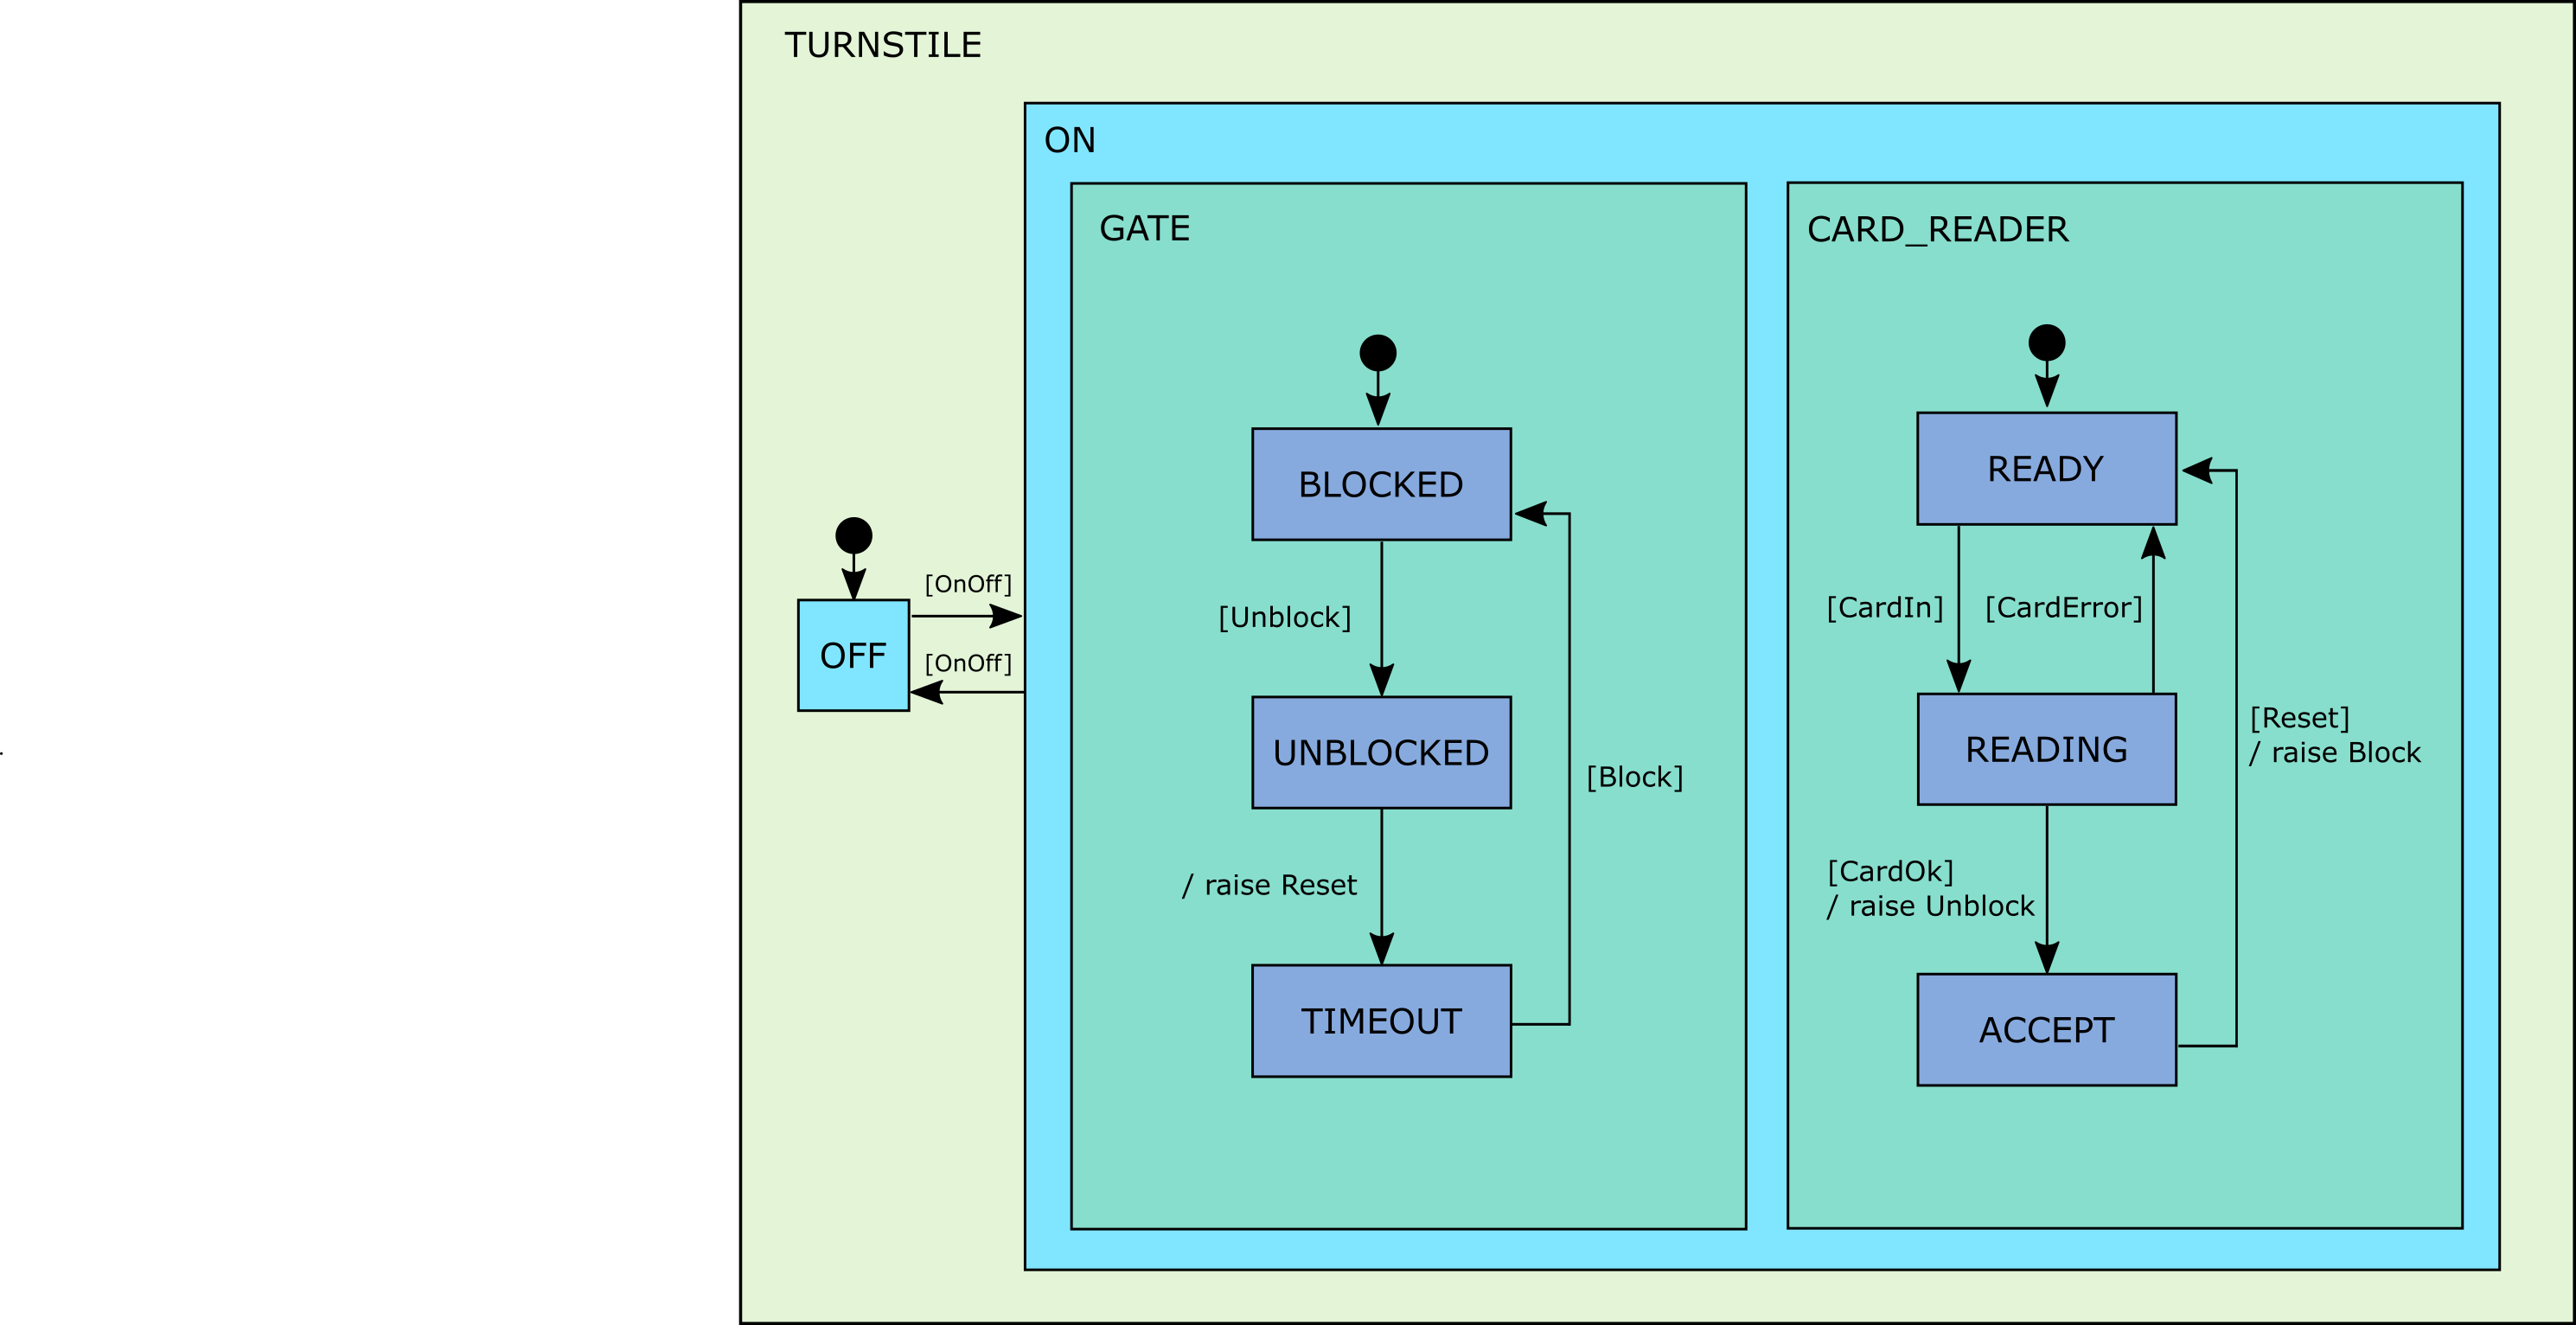
\includegraphics[trim={25cm 0 0 0}, width=0.7\textwidth]{figures/Turnstile.png}
\caption{Design model for a turnstile system}
\label{fig:turnstile}
\end{figure}

The model has two external triggers (\emph{OnOff}, and \emph{CardIn}), which are signals provided by the environment under which the system operates. In addition, there are internal triggers (\emph{CardOk}, \emph{Unblock}, \emph{Block}, and \emph{Reset}) that are raised by the components in the system. In the current model some of the internal triggers are raised non-deterministically (e.g. \emph{CardOk}, \emph{CardError}), as the details of the actual mechanisms responsible for the generation of the signal are not fully specified. Even in the presence of this non-determinism the system must satisfy certain requirements. 
Refinement of the abstract model presented in Figure~\ref{fig:turnstile} can be used to incorporate implementation details. 
For example, a nested  statechart could be added to the \emph{READING} state to specify the process by which the aforementioned triggers are  raised. 
This manuscripts focuses on formalizing the modeling language semantics for triggered statecharts of this form, and leaves the extensions required for refinement proofs to a future publication.  
%The following sections will describe in detailed each of the semantic models constructed to support a specification and formal analysis of this system using our modeling language.
\section{Formalization of Untriggered Statecharts}
\label{sec:utsc}
In this section, we formalise the syntactic elements and semantics of untriggered statecharts.
This  includes finding sufficient conditions for well-defined untriggered statecharts to guarantee consistent semantic behaviour of such models.
The main ideas for our formalisation are 
(1) to use the \EventB \emph{contexts} to capture the \emph{syntactic elements} of the model with axioms ensuring that the model is well-defined (Section~\ref{sec:utsc-syntax}), and 
(2) to use the \EventB \emph{machines} to capture the \emph{semantics} of the models (Section~\ref{sec:utsc-semantics}).

\subsection{Formalisation of the Untriggered Statechart Syntactic Elements}
\label{sec:utsc-syntax}
As the syntactic elements of untriggered statecharts are fairly complex, we develop them gradually, together with their well-definedness conditions,  using \EventB context extension in the following steps.
\begin{enumerate}
    \item Model the tree-structure of the states
    \item Model the parallel regions
    \item Model the transformations between states
\end{enumerate}

\subsubsection{Tree-structure States} The structure of the states of a statechart is represented by  the following constants; |states| (the set of all states), |root| (the implicit root state), |container| (the relationship between a child state and its parent container), |leaves| (the set of leaf states). 
These constants satisfy an axiom stating that they form a tree-shaped structure (here |↦| is the notation for specifying tuples).
\begin{center}
    |states ↦ root ↦ container ↦ leaves ∈ Tree|
\end{center}
Where, |Tree| is a constant, defined using transitive closure, that formalises the definition of tree-shaped structures. 
An important derived property of a tree-shaped structured (proved as a theorem) is needed to allow us to prove properties by induction.
\begin{theorem}[Tree induction from root]
\label{thm:tree-induction}
    Consider a property |P|. If 
    \begin{enumerate}
        \item The |root| satisfies |P|, and
        \item for every non-root state |s|, if the container of |s|, i.e., |container(s)|, satisfies |P|, then |s| also satisfies |P|,
    \end{enumerate}
    then every state in the tree satisfies |P|.
\end{theorem}
%\begin{figure}
%    \centering
%    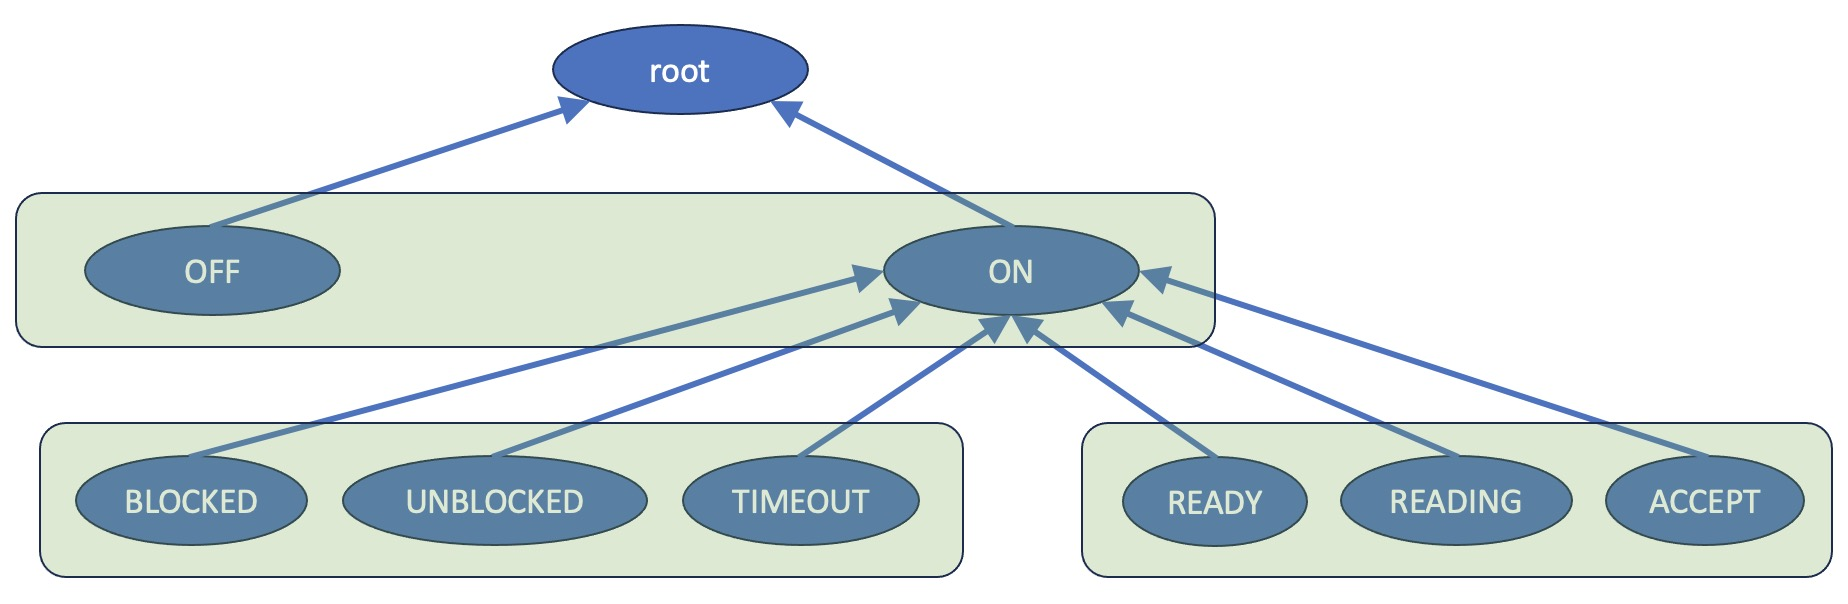
\includegraphics[width=0.8\textwidth]{figures/TreeShapedStates}
%    \caption{The states and regions structure for the turnstile example}
%    \label{fig:turnstile-tree-shaped}
%\end{figure}

\begin{example}[Turnstile Example. Tree-shaped Structure States]
%    The tree-shaped structure of states in the turnstile example can be seen in Figure~\ref{fig:turnstile-tree-shaped}.
    Formally, we have the following definitions.   
\begin{EventBcode}
// All states of the turnstile examples
partition(states, {root}, {OFF}, {ON}, {BLOCKED}, {UNBLOCKED}, {TIMEOUT},
    {READY}, {READING}, {ACCEPT})
// The container relationship between states
container = {OFF ↦ root, ON ↦ root, BLOCKED ↦ ON, UNBLOCKED ↦ ON,
    TIMEOUT ↦ ON, READY ↦ ON, READING ↦ ON, ACCEPT ↦ ON}
// leaf states
leaves = {BLOCKED, UNBLOCKED, TIMEOUT, READY, READING, ACCEPT, OFF}
\end{EventBcode}

The |partition| operator defines an enumerated set, |states|, where all the elements are explicitly given.
\end{example}

\subsubsection{Regions} Untriggered statecharts support the parallel composition of two or more nested statechart regions. 
That is a single state of a statechart may represent several sub components and associate with each component a corresponding region.
In the turnsile example, the container state \emph{ON} has two regions \emph{GATE} and \emph{CARD\_READER}. 
We formalise the notion of regions as partitions of the set of non-root states by using the following axioms to constrain the constant |regions|.

\begin{axiom}[Regions are subsets of states]
\label{axm:@region_type}
Each region is a subset of the statechart's states. (Here |ℙ| is the notation for powerset.)
    \begin{center}
        \EventBInline{@region_type: regions ⊆ ℙ(states)}
    \end{center}
\end{axiom}
\begin{axiom}[Regions are disjoint]
\label{axm:@region_disjoint}
Every pair of distinct regions does not share any states.
    \begin{center}
        \EventBInline{@region_disjoint: !r1, r2 · r1 ∈ regions ∧ r2 ∈ regions ∧ r1 ≠ r2 ⇒ r1 ∩ r2 = ∅}
    \end{center}    
\end{axiom}
\begin{axiom}[Regions cover non-root states]
\label{axm:@region_complete}
Every non-root state belongs to a region.
    \begin{center}
        \EventBInline{@region_complete: union(regions) = states \ \{root\}}
    \end{center}
\end{axiom}
\begin{axiom}[Region has a unique container]
\label{axm:@region_same_parent}
Every region has a unique container state. Here |container[region]| is the image of the relation |container| applying to |region|.
    \begin{center}
        \EventBInline{@region_same_parent: ! region · region ∈ regions ⇒}\\
        \EventBInline{ (∃parent · container[region] = \{parent\})}
    \end{center}
\end{axiom}

\begin{example}[Turnstile Example. Regions]
   % The parallel regions for the turnstile example can be seen in Figure~\ref{fig:turnstile-tree-shaped}.
    Formally, we have three regions as follows.
\begin{EventBcode}
regions = { {ON, OFF}, // TURNSTILE region
	{BLOCKED, UNBLOCKED, TIMEOUT}, // GATE region
	{READY, READING, ACCEPT}	// CARD_READER region
}
\end{EventBcode}
Note that states |ON| and |OFF| implicitly form a region without any sibling parallel region.
\end{example}

\subsubsection{Transformations} Unlike the common definitions of transitions, which map a source state to a target state, we define |transformations|, which give an hierarchical view of the set of all simultaneously enabled transitions of the system, from one \emph{enabling} state configuration to the next configuration. 
There are different types of transformation including 
\emph{forking} (starting from a state and ending in one or more states in different parallel regions), 
\emph{joining} (starting from two or more states in different parallel regions and ending in a state), \emph{parallel} (updating parallel regions at the same time), 
and any combination of these types. 
To model all transformation types, we formalise each transformation by three sets of states.
\begin{itemize}
\item |enabling|: A transformation is enabled (i.e., can be executed)
  if its (non-empty) set of enabling states are active.
  
\item |exiting|: The (possibly empty) set of states that the transformation
  will exit upon execution.
  
\item |entering|: The (possibly empty) set of states the transformation will enter upon
  execution.
\end{itemize}
Formally, these notions are formalised as constants as follows.
\begin{EventBcode}
enabling ∈ transformations → ℙ1(states)
exiting ∈ transformations → ℙ(states)
entering ∈ transformations → ℙ(states)
\end{EventBcode}

\begin{example}[Turnstile Example. Transformation]
We give the enabling, exiting, entering and active states of the following example transformations.
\begin{itemize}
    \item Consider the transformation from the |BLOCKED| state to the |UNBLOCKED| state, we call this |BLOCKED_2_UNBLOCKED|. We have
\begin{EventBcode}
enabling(BLOCKED_2_UNBLOCKED) = {BLOCKED}
exiting(BLOCKED_2_UNBLOCKED) = {BLOCKED}
entering(BLOCKED_2_UNBLOCKED) = {UNBLOCKED}
\end{EventBcode}

    \item Consider the transformation from the |OFF| state to the |ON|
state, we call this |OFF_2_ON|. Notice that the transformation will take into account also the transition from the initial states within the two sub-statecharts (regions). As a result, we have
\begin{EventBcode}
enabling(OFF_2_ON) = {OFF}
exiting(OFF_2_ON) = {OFF}
entering(OFF_2_ON) = {ON, BLOCKED, READY}
\end{EventBcode}

    \item Consider the transformation from the |ON| state to the |OFF|
state, we call this |ON_2_OFF|. Notice that the transformation will take into account the non-deterministic exit from the two sub-statecharts (regions). As a result, we have
\begin{EventBcode}
enabling(ON_2_OFF) = {ON}
exiting(ON_2_OFF) = {ON, BLOCKED, UNBLOCKED, TIMEOUT, READY, READING, ACCEPT}
entering(ON_2_OFF) = {OFF}
\end{EventBcode}
\end{itemize}
\end{example}

There are several additional constraints (well-definedness conditions) relating the enabling, exiting, and entering states for a transformation. We identified some of the constraints directly. For instance, the following axioms related to |exiting| states.
\begin{axiom}[Exiting a contained region]
\label{axm:@exiting-contained_region}
If the container of a region is an exiting state, there must be an exiting state within that region. Here |container[r]|, is the image of the relation container applying to region |r|.
\begin{EventBcode}
@exiting-contained_region:
    ∀trf, s, r · trf ∈ transformations ∧ s ∈ exiting(trf) ∧ r ∈ regions ∧ container[r] = {s}
        ⇒ exiting(trf) ∩ r ≠ ∅
\end{EventBcode}
\end{axiom}

\begin{axiom}[Exiting one or all states in a region]
\label{axm:@exiting-either_one_or_all_in_a_region}
If a region |r| has an exiting state |s| then either |s| is the unique exiting state or all the states in |r| are exiting states.
\begin{EventBcode}
@exiting-either_one_or_all_in_a_region: 
    ∀trf, s, r · trf ∈ transformations ∧ s ∈ exiting(trf) ∧ r ∈ regions ∧ s ∈ r
        ⇒ exiting(trf) ∩ r = {s} ∨ r ⊆ exiting(trf)
\end{EventBcode}
\end{axiom}

The following axioms linking |exiting| and |enabling| states was ``discovered'' during the proof of the invariant preservation proof obligations (see Theorem~\ref{po:transformation/active_container/INV}).
\begin{axiom}[Exiting a unique enabling state in a region]
\label{axm:@exiting-unique_enabling_state_in_a_region}
Given a region |r| and an exiting state |s| in |r|, if |r| has states other than |s|, |s| must be the unique enabling state in |r|.
\begin{EventBcode}
@exiting-unique_enabling_state_in_a_region:
    ∀trf, s, r · trf ∈ transformations ∧ r ∈ regions ∧ exiting(trf) ∩ r = {s} ∧ r ≠ {s}
        ⇒ enabling(trf) ∩ r = {s}
\end{EventBcode}
\end{axiom}
\begin{axiom}[Enabling state is the unique exiting state]
\label{axm:@enabling-unique_exiting_state_in_a_region}
Given a region |r| with some exiting state, an enabling state |s| in |r|, |s| must the unique exiting state in |r|.
\begin{EventBcode}
@enabling-unique_exiting_state_in_a_region:
    ∀trf, s, r · trf ∈ transformations ∧ s ∈ enabling(trf) ∧
    exiting(trf) ∩ r ≠ ∅ ∧ r ∈ regions ∧ s ∈ r ⇒ exiting(trf) ∩ r = {s}
\end{EventBcode}
\end{axiom}

The following axiom relates |entering| with |enabling| and |exiting| states. It is also discovered during the proof of the invariant preservation proof obligations (see Theorem~\ref{po:transformation/active_container/INV}).
\begin{axiom}[Transformation stays within a state]
\label{axm:@entering-stay_within_state}
If a transformation enters a region |r| but not the container of |r| (called |c|), then |c| is not an exiting state and there is an enabling state which is a descendant of |c|. Here, |cl(container)| denote the transitive closure of |container| relationship, hence the inverse of that (i.e., |cl(container)∼| is the descendant relationship between states.
\begin{EventBcode}
@entering-stay_within_state:
    ∀trf, r, c · trf ∈ transformations ∧ r ∈ regions ∧ container[r] = {c} ∧
    entering(trf) ∩ r ≠ ∅ ∧ entering(trf) ∩ container[r] = ∅
        ⇒ enabling(trf) ∩ cl(container)∼[{c}] ≠ ∅ ∧ c ∉ exiting(trf) 
\end{EventBcode}
\end{axiom}


\subsection{Formalisation of the Untriggered Statechart Semantics}
\label{sec:utsc-semantics}

Given an untriggered statechart (characterized by the tree-shape structured states, the regions, and the transformation), the semantics of the statechart is characterized by the set of active states during its execution. For instance, consider the turnstile example in Figure~\ref{fig:turnstile}, initially, the turnstile has one active state, namely |OFF|, i.e., the set of active states is |{OFF}|
\begin{itemize}
    \item A transformation |OFF_2_ON| (from |OFF| to |ON|) will change the set of active states to |{ON, BLOCKED, READY}|.
    \item A transformation |BLOCKED_2_UNBLOCKED| will change the set of active states to |{ON, UNBLOCKED, READY}|.
    \item A transformation |ON_2_OFF| changes the set of active states to |{OFF}|.
\end{itemize}

We can now formalize the semantics of the untriggered statechart in a machine using a single variable |active| satisfying |active ⊆ states|. 
The system's functionality is encoded through one event called |transformation| that captures how the design transitions from one configuration to the next. 
Essentially variable |active| provides a discrete characterization of the information and event |transformation| represents the operation of the system under analysis. 
\begin{EventBcode}
event transformation
any trf where
	@typeof-trf: trf ∈ transformations
	@active-enabling: enabling(trf) ⊆ active
then
	@update-active: active ≔ (active ∖ exiting(trf)) ∪ entering(trf)
end
\end{EventBcode}
Guard |@active-enabling| ensures that the chosen transformation |trf| is enabled and action |@update-active| first removes the |trf|'s exiting states then adds |trf|'s entering states.  Notice that this action also allows a transformation to exit a state and re-enter that state.

An important aspect for the semantics of statecharts is that it can only transform amongst valid configurations.  For example, we want to ensure that the turnstile statechart is never in the configuration where both |ON| and |OFF| states are active or in a state where |BLOCKED| is active, but |ON| is not active. The following constraints on |active| specify the valid configuration for a statechart, which we encode as 4 invariants for the machine.
\begin{invariant}[Container active]
\label{inv:container_active}
If a non-root state is active then its container is also active.
\begin{center}
\EventBInline{@container_active: ∀ s · s ∈ active ∖ {root} ⇒ container(s) ∈ active}
\end{center}
\end{invariant}
\begin{invariant}[Content active]
\label{inv:content_active}
If a container state is active then one of its sub-state must be active.
\begin{center}
\EventBInline{@content_active: ∀ s · s ∈ ran(container) ∧ s ∈ active ⇒}\\
\EventBInline{container∼[\{s\}] ∩ active ≠ ∅}
\end{center}
where |ran(container)| is the range of the container relation
\end{invariant}
\begin{invariant}[Unique active state within a region]
\label{inv:active-region-unique}
There can be at most one active state in a region.
\begin{center}
\EventBInline{@active-region-unique: ∀r, s · r ∈ regions ∧ s ∈ r ∩ active ⇒ r ∩ active ⊆ \{s\}}
\end{center}
\end{invariant}
\begin{invariant}[Parallel regions are inactive/active at the same time]
\label{inv:active-region-parallel}
All parallel regions are inactive (hence active) at the same time.
\begin{center}
\EventBInline{@active-region-parallel: ∀r1, r2 · r1 ∈ regions ∧ r2 ∈ regions ∧} \\
\EventBInline{container[r1] = container[r2] ∧ r1 ∩ active = ∅ ⇒ r2 ∩ active = ∅}
\end{center}
\end{invariant}
As a consequence of Invariant~\ref{inv:container_active}, we can prove the following machine theorem. Note that all proofs related to this work were discharged semi-automatically within Rodin using the Proving Perspective. We present the general structure of a selected subset of these proofs.
\begin{theorem}[Ancestors active]
\label{thm:@ancestor_active}
If a state |s| is active then all ancestors of |s| are also active.
\begin{center}
\EventBInline{@ancestor_active:	∀ s · s ∈ active ⇒ cl(container)[{s}] ⊆ active}
\end{center}
\end{theorem}
\begin{proof}
The proof of the theorem relying on Invariant~\ref{inv:container_active} and the inductive nature of transitive closure. We omit the details here.
\end{proof}

We have to prove that event |transformation| maintains the  invariants relying on the well-definedness constraints that we have put as axioms.

%The majority of the proof obligations generated by the Rodin tool are automatically discharged. In the following section we illustrate the proof to ensure that if a state is active its corresponding container must also be active. This invariant is defined in property~\ref{container_active}. 
%Additional invariants that required manual proofs are related to ensuring the only one state is active in any active region, invariant~|@active-region-unique|).

\subsubsection{Preservation of invariant \EventBInline{@active_container}}
%The semantics of this modeling language requires that for any model constructed, the container for any active state must itself be active. This property is capture in invariant~\ref{container_active}. 
The proof obligation for ensuring that invariant |@active_container| is maintained by event |@transformation| after simplification can be stated as the following theorem.
\begin{theorem}[Event \EventBInline{transformation} maintains \EventBInline{@active_container}]
\label{po:transformation/active_container/INV}
Given a non-root state |s| such that either (1) |s| is active but non−exiting state, or (2) |s| is an entering state, then either (G1) |container(s)| is active but non-exiting state, or (G2) |container(s)| is an entering state.
\end{theorem}

\begin{proof}
 Since |s| is a non-root state, there exists a region |r| containing |s| (follows from Axiom~\ref{axm:@region_complete} |@region_complete|). 
We continue the proof by considering Cases~\ref{container_active:case1} and Case~\ref{container_active:case2}.
\begin{case}[\EventBInline{s} is active but non-exiting state]
\label{container_active:case1}
We discharge (G1) by proving that (G1-1) |container(s)| is an active state, and (G1-2) |container(s)| is a non-exiting state.
\begin{itemize}
\item \emph{Proof of (G1-1)}. According to Invariant~\ref{inv:container_active} (|@container_active|), since |s| is an active state, |container(s)| is an active state.

\item \emph{Proof of (G1-2)}. We proceed by considering if |r| contains any exiting states.
    \begin{itemize}
        \item \emph{Case 1.1 (\EventBInline{r} does not contain any exiting states)} Using the contraposition of Axiom~\ref{axm:@exiting-contained_region}, we can conclude that |container(s)| (which is also the container of the region |r|) must not be an exiting state, which conclude the proof of (G1-2).

        \item \emph{Case 1.2 (\EventBInline{r} contains some exiting states)} The proof continue as follows.
            \begin{itemize}
            \item According to Axiom~\ref{axm:@enabling-unique_exiting_state_in_a_region} (|@enabling-unique_exiting_state_in_a_region|), |s| cannot be an enabling state since |s| is a non-exiting state.

            \item We prove this by contradiction, i.e., assuming that |container(s)| is an exiting state.
                \begin{itemize}
                    \item According to Axiom~\ref{axm:@exiting-contained_region} (|@exiting−contained_region|), there must be an exiting state in the region |r| since the state containing |r| (in this case |container(s)|) is an exiting state, let us call this state |x|.

                    \item According to Axiom~\ref{axm:@exiting-either_one_or_all_in_a_region} (|@exiting-either_one_or_all_in_a_region|, either |x| is the unique exiting state in |r| or all states in |r| are exiting states.

                    \item Since |s| is a non-exiting state, |x| must be |r|'s unique exiting state.

                    \item From Axiom~\ref{axm:@exiting-unique_enabling_state_in_a_region} (|@exiting-unique_enabling_state_in_a_region|), |x| is the unique enabling state in |r|.

                    \item According to guard |@active-enabling| of |transformation|, |x| (being an enabling state) must be an active state.

                    \item We now have two distinct active states |x| and |s| in |r|, which contradicts Invariant~\ref{inv:active-region-unique} (|@active-region-unique|).
                \end{itemize}
            \end{itemize}
        \end{itemize}
    \end{itemize}
\end{case}

\begin{case}[\EventBInline{s} is an entering state]
\label{container_active:case2}
In this case, we proceed with the proof by assuming that (G2) does not hold (i.e., |container(s)| is not a container state) and prove (G1).  
\begin{itemize}
    \item According to Axiom~\ref{axm:@entering-stay_within_state}, the transformation entering region |r| but not the container of |r| (i.e., |container(s)|), hence |container(s)| is not an exiting state and has a enabling descendant state, let us call this |x|.

    \item According to guard |@active-enabling| of |transformation|, |x| (being an enabling state) must be an active state.
    
    \item According to Theorem~\ref{thm:@ancestor_active}, |container(s)| (being an ancestor of |x|) must be an active state. 

    \item We therefore have |container(s)| is active but non-exiting state (G1).    
\end{itemize}
\end{case}
\qed
\end{proof}
        

% \subsubsection{Proof obligation for active content within a container}

% For all s where 
%       (H1) s is a container state and
%        s is (H2·1) active and NOT exiting state OR
%             (H2·2) s is an entering state
%   then
%       there exists a child state of s which is either
%        (G1) active and NOT existing state OR
%        (G2) an entering state

% Consider proof by cases for (H2·1) and (H2·2)

% (H2·1), i·e·, s is active and NOT exiting state
%   − Instantiate INV @content_active, we have
%     there exist a child state of s which is active, call this child state x
%   − Consider proof by case on x is an exiting state OR ¬
%     (a) x is an exiting state
%         + We first prove that there exists a child state of s which is an entering state
%            −− There exists a region r contains x
%               ==== TBA ====
%            −− r ◁ container=r × {s}, i.e., every state in r must have
%           s as its container.
%               === TBA ===
%            −− Instantiating @entering−you_must_go*somewhere with r, we
%            obtain that there must be an entering state within r
%         + Let's call this child state x0, which is an entering state·
%            x0 is a candidate for (G2)
%     (b) x is NOT an exiting state
%         x would be a candidate for (G1)
 
% (H2·2) i·e·, s is an entering state
%    − There exists a region r contained in s, i·e·, ∃ r   · r∈regions ∧r ◁ container=r × {s}
%           ==== TBA ====
%    − Instantiate AXM @entering−contained*region,
%        we obtain that there is an entering state in r, i·e·, entering(trf) ∩ r ≠ ∅
%        we call this entering state in r x and 
%        we will prove that x is a candidate for either (G1) OR (G2)

%The untriggered statechart component of the turnstile example consists of a Event-B context which includes constants for all states in the model and hierarchical information is capture via axioms that define container relations and leaves states in the design (see context utstc\_ctx0\_turnstile in ~\cite{supporting-data}).

We omit the proof of the preservation of other Invariants~\ref{inv:content_active}, \ref{inv:active-region-unique}, and \ref{inv:active-region-parallel} due to limited space. 
The proofs is done within the Rodin tool utilising several axioms and the tree induction theorem (Theorem~\ref{thm:tree-induction}). 
Details can be found in~\cite{Hoang2023:SCXMLSemanticsModel}.

%%% Local Variables:
%%% mode: latex
%%% TeX-master: "../main"
%%% End:
\section{Formalization of the Run-to-Completion Schedule}
\label{sec:r2c}
Similar to the previous section, the formalization is done using an \EventB context to capture the syntactic elements (Section~\ref{sec:r2c-syntax}) and an \EventB machine to model the semantics (Section~\ref{sec:r2c-semantics}).

\subsection{Formalization of the Run-to-completion Syntactic Elements}
\label{sec:r2c-syntax}
To define run to completion execution we first specify the  syntactic elements involved. 
Triggers, are partitioned into either  Internal or External triggers.
%\begin{center}
%    \EventBInline{partition (TRIGGERS, InternalTriggersType, ExternalTriggerType, {nullTrigger})}
%\end{center}
We define the internal and external trigger queues as sequences of internal and external triggers respectively. Sequences and their allowed operations (e.g. append trigger, head of sequence) are constructively defined via a series of theorems and axioms which are omitted here.

%A null trigger |nullTrigger| is introduced for convenience to simplify the 
%definition of the initial condition. As shown in 
%Figure~\ref{fig:run-to-completion} shows the execution begins by taking untriggered steps which is otherwise only done after a trigger is consumed. Hence the |nullTrigger| is said to be consumed during initialization.
Figure~\ref{fig:run-to-completion} shows the state machine for the run-to-completion schedule. 
From the \emph{Ready to de-queue} state, an internal or (if internal queue empty) external trigger is de-queued from the corresponding queues and the system moves to the \emph{Firing Triggered} state.
A trigger step that consumes the dequeued trigger is then fired and the system moves to the \emph{Firing Untriggered} state. 
From this state, untriggered steps can be fired repeatedly or the system moves back to the \emph{Ready to de-queue} state. 
Both triggered and untriggered steps can raise more internal triggers, which will need to be handled in the future runs.
\begin{figure}[!t]
\centering
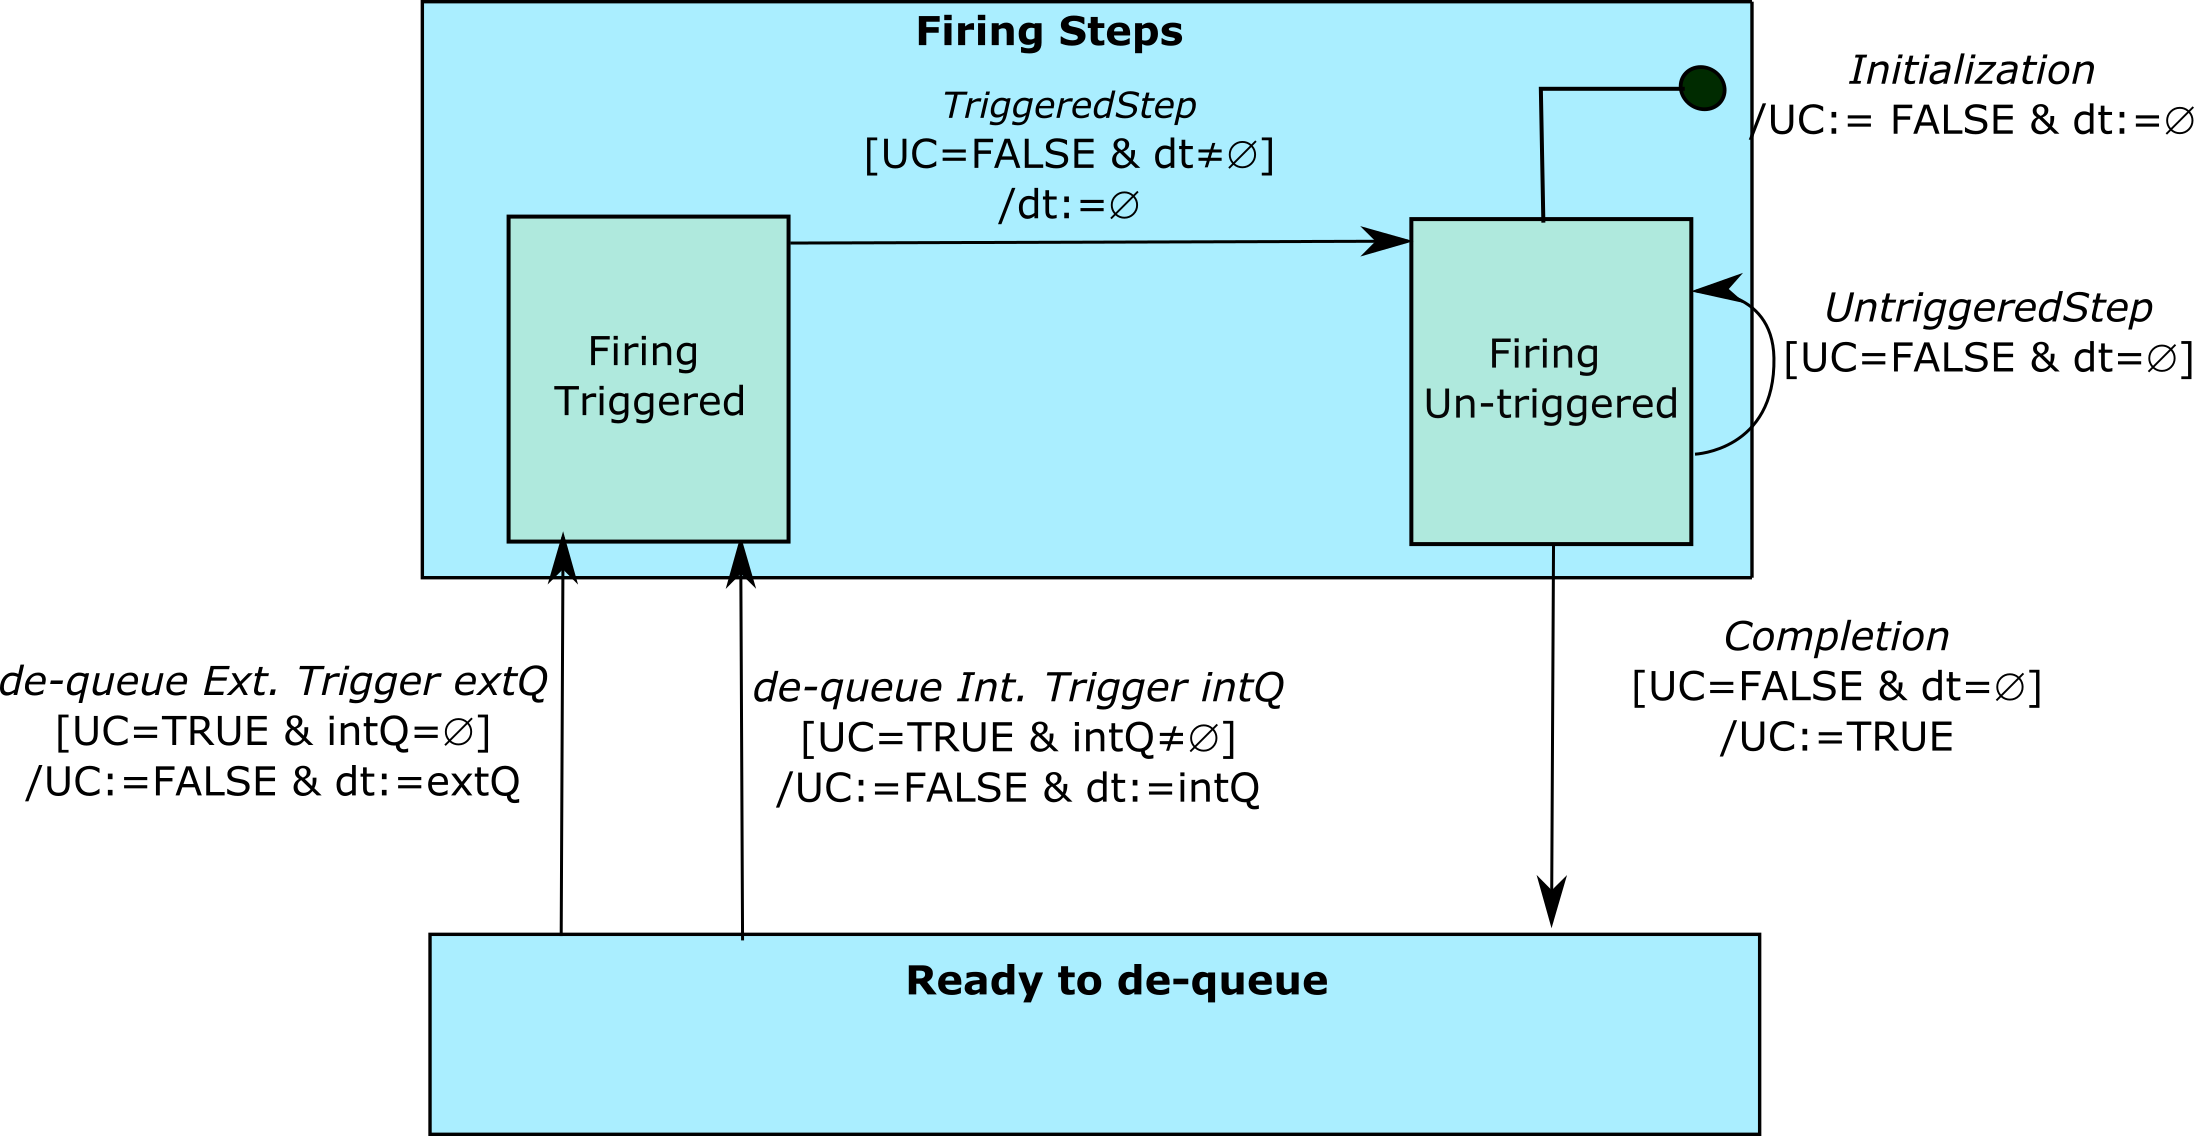
\includegraphics[width=0.7\textwidth]{figures/run-to-completion.png}
\caption{State diagram for run to completion scheduling}
\label{fig:run-to-completion}
\end{figure}

The context defining the syntactic elements for a run to completion is shown in Listing~\ref{lst:r2c_ctx}. 
An important notion for the run to completion schedule are steps.  
A triggered  step is taken when an internal or external trigger is consumed and a non-deterministic number of untriggered steps may be taken after a triggered step. 
In the next section we will show how these steps relate to triggered and untriggered transitions  

\begin{lstlisting}[language=Event-B, caption = {Context for Run-to-Completion Semantics}, label = {lst:r2c_ctx}]
context r2c_ctx
extends r2c_c0_2_dequeue 
sets Steps
constants InternalTriggers ExternalTriggers Triggers StepTrigger StepRaised
axioms
	@typeof_IT: InternalTriggers ⊆ InternalTriggerType
	@typeof_XT: ExternalTriggers ⊆ ExternalTriggerType
	@def_T: Triggers = InternalTriggers ∪ ExternalTriggers
	@typeof_StepTrigger: StepTrigger ∈ Steps ⇸ Triggers
	@typeof_StepRaised: StepRaised ∈ Steps → Seq(InternalTriggers)
end
\end{lstlisting} 
Here |StepTrigger| (as a partial function) defines the required trigger for a Step (if any), and |StepRaised| defines the sequence of internal triggers that will be raised for a step (including an empty sequence). Steps that do not have any required trigger will be untriggered steps.

\subsection{Formalization of the Run-to-Completion Semantics}
\label{sec:r2c-semantics}
Given the syntactic elements defined earlier, the machine defining the semantics for the run-to-completion schedule models the trigger queues in the system according to Figure~\ref{fig:run-to-completion}. The dynamic status of the run-to-completion schedule is represented by the variables |int_q|, |ext_q|, |dt| (dequeue trigger), and |completion| with the following invariants.
\begin{EventBcode}
	@int_q: int_q ∈ Seq(InternalTriggers)
	@ext_q: ext_q ∈ Seq(ExternalTriggers)
	@dequeue_trigger: dt ∈ DeQueueType
	@dequeue_triggerwd:	dt ⊆ InternalTriggers ∪ ExternalTriggers
	@firingTriggered: dt ≠ ∅ ⇒ completed=FALSE
\end{EventBcode}
Where |int_q| and |ext_q| represent the sequences of internal and external triggers that need to be handled, |dt| keeps track of the trigger that has been removed from the queues (de-queue) to be consumed by a |TriggeredStep|. Note that |dt| is a singleton set of trigger when the system is in the \emph{Firing Triggered} state and empty otherwise (this is also the definition of |DeQueueType|). Finally, variable |complete| (denoted as |UC| in Figure~\ref{fig:run-to-completion}) is |TRUE| indicates that the system is in the \emph{Ready to de-queue} state.

Starting from the \emph{Ready to de-queue} state (where |completed = TRUE|), the system will de-queue an internal/external trigger if there are any. Note that an external trigger is only de-queued when the internal queue is empty. After that the system moves to the \emph{Firing triggered} state (where |completed = FALSE| and |dt| is no longer empty).
\begin{center}
\begin{minipage}[t]{0.48\textwidth}
\begin{EventBcode}
event dequeueInternalTrigger
any trigger where 
	@grd1: completed = TRUE
	@grd2: int_q ≠ ∅
	@grd3: trigger = Seq_head(int_q)
then 
	@act1: dt ≔ {trigger}
	@act2: int_q ≔ Seq_tail(int_q) 
	@act3: completed ≔ FALSE
end
\end{EventBcode}
\end{minipage}
\hfill
\begin{minipage}[t]{0.48\textwidth}
\begin{EventBcode}
event dequeueExternalTrigger
any trigger where 
    @grd1: completed = TRUE
    @grd2: ext_q ≠ ∅
    @grd3: trigger = Seq_head(ext_q)
    @grd4: int_q = ∅
then 
    @act1: dt ≔ {trigger}
    @act2: ext_q ≔ Seq_tail(ext_q)
    @act3: completed ≔ FALSE
end
\end{EventBcode}
\end{minipage}
\end{center}

The behaviour of the \emph{TriggeredStep} and \emph{UntriggeredStep} are formalised by the corresponding events as follows. Both events can raise a sequence of internal triggers which is concatenated to the the internal queue.
\begin{center}
    \begin{minipage}[t]{0.48\textwidth}
\begin{EventBcode}
event triggeredStep 
any Step where 
    @grd1: Step ∈ dom(StepTrigger)		
    @grd2: StepTrigger(Step) ∈ dt
then 
    @act1: dt ≔ dt ∖ {StepTrigger(Step)}
    @act2: int_q ≔ Seq_concat(int_q ↦ StepRaised(Step))
end
\end{EventBcode}
    \end{minipage}
    \hfill
    \begin{minipage}[t]{0.51\textwidth}
\begin{EventBcode}
event untriggeredStep 
any Step where 
    @grd1: Step ∈ Steps ∖ dom(StepTrigger)	
    @grd2: dt = ∅
then 
	@act1: int_q ≔ Seq_concat(int_q ↦ StepRaised(Step))
end
\end{EventBcode}
    \end{minipage}
\end{center}
While the internal triggers are raised through steps, external triggers can be raised non-deterministically by event |raiseExternalTrigger| and appended to the external queue. 
%Finally, the system can complete when there are no dequeue trigger. 
Note that at this stage (without the statemachine), there is a non-determinism between |untriggeredStep| and |completion|. 
When we combine the untriggered statechart and the run-to-completion schedule in the next section, we will distinguish the two cases.
\begin{center}
    \begin{minipage}[t]{0.55\textwidth}
\begin{EventBcode}
event raiseExternalTrigger
any trigger where
    @grd1: trigger ∈ ExternalTriggers
then
    @act1: ext_q ≔ Seq_append(ext_q ↦ trigger)
end
\end{EventBcode}
    \end{minipage}
    \hfill
    \begin{minipage}[t]{0.43\textwidth}
\begin{EventBcode}
event completion
where
    @grd1: dt = ∅
    @grd2: completed = FALSE
then
    @act1: completed ≔ TRUE
end
\end{EventBcode}
    \end{minipage}
\end{center}

The model of the run-to-completion schedule maintains its invariants straightforwardly (relying on operations of sequence manipulation).
\section{Formalization of Triggered Statecharts}
\label{sec:tstc}

The triggered statecharts is an unified statechart model representation based 
on SCXML ~\cite{scxmlwebsite}. To formalize the complete semantics we compose the previous two models, of the untriggered statechart (Sections~\ref{sec:utsc}) and of the run-to-completion schedule (Section~\ref{sec:r2c}).
The composition is performed by, using the inclusion mechanism built into the CamilleX extension~\cite{DBLP:conf/sefm/HoangSDFB22} of the Rodin platform.

\subsection{Triggered Statechart Syntactic Elements}
\label{sec:tstc-syntax}
Since the a triggered statechart is a combination of its untriggered statechart and the run-to-completion schedule, the syntactic elements of triggered statechart extend the syntactic elements of the untriggered statechart and the run-to-completion (Listing~\ref{lst:tstc_ctx}). We introduce some syntactic elements \emph{gluing} the sub-context together, namely, the link between untriggered statechart's transformations and run-to-completion's steps, to form |transitions|.

At the same time, when we combine the two sub-models, we need to ensure an important aspect of triggered statecharts which is their responsiveness. In particular, if a trigger (internal or external) is de-queued, but no enabled transformation that can consume the trigger, we need to ensure that the system can still progress. More precisely, the system will need to \emph{discard} the problematic trigger in order to continue. Constants |discardSteps| are introduced to capture the special steps that discarding triggers.

Axiom |@typeof-transitions| specifies that |transitions| is a one-to-one correspondence between transformations and non-discarding steps (|⤖| is the symbol for bijective functions). Axioms |@discardSteps-Triggers| and |@discardSteps-Raised| ensure that there is a discard step for every trigger and the discard steps do not raise any trigger.
\begin{lstlisting}[language=Event-B, caption = {Context for Triggered Statecart}, label = {lst:tstc_ctx}]
context tstc_ctx
extends r2c_ctx utstc_ctx
constants transitions discardSteps
axioms
	@typeof-transitions: transitions ∈ transformations ⤖ Steps ∖ discardSteps
	@discardSteps-Triggers: discardSteps ◁ StepTrigger ∈ discardSteps ⤖ Triggers
	@discardSteps-Raised: StepRaised[discardSteps] = { ∅ }
end
\end{lstlisting}

\subsection{Triggered Statechart Semantics}
\label{sec:tstc-semantics}
The semantics of a triggered statechart is capture by a machine that includes both the untriggered statechart and the run-to-completion schedule. We also use prefixing mechanism, e.g., |as r2c|, so that all modelling elements of the included machine are prefixed accordingly.
\begin{EventBcode}
machine tstc sees tstc_ctx
includes r2c as r2c
includes utstc as utstc
\end{EventBcode}
The following events are \emph{lifted} from the run-to-completion machine (unchanged): |raiseExternalTrigger|, |dequeueExternalTrigger|, |dequeueInternalTrigger|. Essentially, they only concern the management of trigger queues and do not relate to the statechart's status.

Events to model the transitions (|triggeredTransition| and |untriggeredTransition|) \emph{synchronises} with the events from the untriggered statechart and the run-to-complete schedule. The additional guard of the events ensure that the chosen tranformation (from the untriggered statechart) and the step (from the run-to-completion model) corresponds with each other.
\begin{center}
    \begin{minipage}{0.48\textwidth}
\begin{EventBcode}
event triggeredTransition
synchronises r2c.triggeredStep
synchronises utstc.transformation
where 
	@grd1: transitions(utstc_trf) = r2c_Step 
end
\end{EventBcode}
    \end{minipage}
    \hfill
    \begin{minipage}{0.48\textwidth}
\begin{EventBcode}
event untriggeredTransition
synchronises r2c.untriggeredStep
synchronises utstc.transformation
where 
	@grd1: transitions(utstc_trf) = r2c_Step 
end    
\end{EventBcode}
    \end{minipage}
\end{center}

As discussed before, we need to introduce the events to discard triggers |discardTrigger| (in the case where |triggeredTransition| is not available). This condition is formalised as  |discardTrigger|'s |grd3|. We also strengthen the guard of |completion| to ensure that the system will complete a run only when |untriggedTransition| is not available (see |completion|'s |grd1|.
\begin{center}
    \begin{minipage}[t]{0.50\textwidth}
\begin{EventBcode}
event discardTriggered
any trigger
synchronises r2c.triggeredStep
where
    @grd1: r2c_Step ∈ discardSteps
    @grd2: trigger = StepTrigger(r2c_Step)
    @grd3: ∀trf · transitions(trf) ∈ StepTrigger∼[{trigger}] ⇒ ¬enabling(trf) ⊆ utstc_active  
end
\end{EventBcode}
    \end{minipage}
    \hfill
    \begin{minipage}[t]{0.48\textwidth}
\begin{EventBcode}
event completion
synchronises r2c.completion
where
    @grd1: 
        ∀ r2c_Step · r2c_Step ∈ Steps ∖ dom(StepTrigger)
	⇒
    ¬ (enabling(transitions∼(r2c_Step)) ⊆ utstc_active)
	end
\end{EventBcode}
    \end{minipage}
\end{center}

Using composition via inclusion mechanism means that the triggered statechart semantics inherit the invariants from the sub-machines without the need to prove them (correct-by-construction).

% \subsection{Machine 1: Composition of SCXML and statemachine }
% For this stage we include the corresponding M1 stages for SCXML and state-machine.

% The gluing context defines the needed refinement relationship between concrete and abstract parts of the model.
% \begin{enumerate}
% 	\item \label{item:triggeredness} For transitions that refine abstract transitions, the transition is triggered if and only if its corresponding abstract transition is triggered.
% 	\item For \emph{triggered} transitions that refine abstract transitions, the trigger is the same as that of the corresponding abstract transition.
% 	\item For \emph{finalized} transitions that refine abstract \emph{finalized} transitions, the transition source is the same as that of the corresponding abstract transition. I.e. you cannot strengthen the source of an already finalised transition.
% 	\item the abstract \emph{finalised} transitions are a subset of the abstract transitions that correspond to concrete finalized transitions. I.e. once transitions are finalized they stay finalized in refinements. 
% \end{enumerate}
% Initially, for item \ref{item:triggeredness} we defined a single axiom giving the equality of the domains of the abstract and concrete transition-trigger relationship.
% However, this was insufficient to prove the guard strengthening of the untriggered refined transitions because the \emph{transition\_link} relationship is not injective. In general, an abstract transition could be refined by more than one concrete transition. We defined two axioms, universally quantifying over the set of refined transitions that are/are not triggered, with the consequent that the corresponding abstract transitions are/are not triggered.
% These axioms were sufficient to automatically discharge the guard strengthening POs for both triggered and untriggered refined transitions.

% \subsection{Machine 2: Merging Abstract and Concrete Events}
% We found a problem when we tried to merge the refined and new  transitions of the combined scxml and statechart semantics. 
% The problem occurs for merging both triggered and untriggered transitions.
% The problem is that we have not considered the case of merging a new state-machine transition with an old refined scxml triggered transition.
% Probably this is nonsensical and we should add guards to prevent it.
% Ok for triggered but for untriggered our way of distinguishing refined scxml untriggered transitions is via the disappearing variable dqaux

% \begin{EventBcode}\caption{Machine for Triggered Statechart Semantics} \label{lst:trigger_stm_mach}
% machine tstc
% sees tstc_ctx
% includes r2c as r2c
% includes utstc as utstc

% events
% 	event INITIALISATION
% 	synchronises r2c.INITIALISATION
% 	synchronises utstc.INITIALISATION
% 	end

% 	event raiseExternalTrigger
% 	synchronises r2c.raiseExternalTrigger
% 	end
	
% 	event dequeueExternalTrigger
% 	synchronises r2c.dequeueExternalTrigger
% 	end
	
% 	event dequeueInternalTrigger
% 	synchronises r2c.dequeueInternalTrigger
% 	end
	
	
% 	event discardTriggered
% 	any trigger
% 	synchronises r2c.triggeredStep
% 	where
% 		// r2c_Step is a discard step
% 		@Step-discard: r2c_Step ∈ discardSteps
% 		// trigger is the discard trigger
% 		@trigger-def: trigger = StepTrigger(r2c_Step)
		
% 		// for all transformation @trf that is triggered by @trigger is disabled,
% 		// i.e., not all enabling states of @trf is active.
% 		@no_enabling: ∀trf · transitions(trf) ∈ StepTrigger∼[{trigger}] ⇒ ¬enabling(trf) ⊆ utstc_active  
% 	end

% 	event triggeredTransition
% 	synchronises r2c.triggeredStep
% 	synchronises utstc.transformation
% 	where 
% 		@this_trigger:	transitions(utstc_trf) = r2c_Step 
% 	end

% 	event untriggeredTransition
% 	synchronises r2c.untriggeredStep
% 	synchronises utstc.transformation
% 	where 
% 		@this_trigger:	transitions(utstc_trf) = r2c_Step 
% 	end

% 	event completion
% 	synchronises r2c.completion
% 	where
% 		// This theorem is useful for discharging no_enabling/WD PO
% 		theorem @COPY-typeof-transitions: transitions∈transformations ⤖ Steps ∖ discardSteps

% 	 	// For all untriggered step r2c_Step, the corresponding transformation, 
% 		// i.e., transitions∼(r2c_Step) is not enabled.
% 		@no_enabling: 
% 			∀ r2c_Step · r2c_Step ∈ Steps ∖ dom(StepTrigger)
% 		⇒
% 			¬ (enabling(transitions∼(r2c_Step)) ⊆ utstc_active)
% 	end
% \end{EventBcode}

%\input{sections/relatedwork.tex} % Add a subsection in the intro to include related work
\section{Conclusions}
\label{sec:conclusions}

In this paper, we formalize the semantics of SCXML run-to-completion statecharts using \EventB. We formalize the syntactic elements using \EventB contexts and using \EventB machines to model the dynamic semantics.  Moreover the semantics model is built in a compositional fashion: the semantics of (untriggered) statechart and run-to-completion schedule is developed independently and composed to create the SCXML statechart's semantics model. This approach allows us to reduce the complexity on the consistency reasoning by focusing on the different parts of the models. The combined model inherits the consistency of the sub-models by construction.

In order to ensure the consistency of the semantics, several well-definedness conditions on the syntactic elements have been identified. They are encoded as axioms in the formal models. These well-definedness conditions can be used as the specification of a validation tool to ensure the consistency of SCXML models. Given the semantic model are consistent, any instantiation will inherit this consistency without the need for reproving. For instance, the model of the turnstile example can have consistency about the active states and the triggering mechanism. Often, these consistency checks make up the majority of the proof  obligations, and only a small number are related to the specific properties of the model.

% Future work
We plan to extend this work to  accommodate for the semantics of refinement as described in~\cite{Morris2018,Morris2020}. In particular, we will formalise the syntactic constraints which allow the consistent refinement of SCXML run-to-completion statecharts, proving the consistency of the refinement rules, e.g., in \cite{DBLP:journals/isse/MorrisSHHAB22}.  The consistency of the semantic models focuses on safety properties, expressed as invariants. Furthermore, we model some of the syntactic elements in our formal models at a fairly abstract level, e.g., the notion of |enabling|, |exiting|, |entering| states for transformation.  This means that the model can be applied to different statechart notations, e.g. UML-B~\cite{DBLP:conf/sefm/SnookBHFD22}.
%At the moment, our semantics focuses on the statemachine structure and the run-to-completion mechanism. We will extend this semantics model to cover other aspects of the notation such as data items.

\vspace{6 pt}
\begin{scriptsize}
	
	\par
	\noindent
	All data supporting this study are openly available from the University of Southampton repository at \url{https://doi.org/10.5258/SOTON/D2791}.\\ 
    \label{public-data}

	\par
	\noindent
	\textbf{Acknowledgements} Sandia National Laboratories is a multimission laboratory managed and operated by National Technology \& Engineering Solutions of Sandia, LLC, a wholly owned subsidiary of Honeywell International Inc., for the U.S. Department of Energy’s National Nuclear Security Administration under contract DE-NA0003525.
	
\end{scriptsize}

\bibliographystyle{plain}
\bibliography{ictac2023}

\end{document}
